
\section{分析結果}

\subsection{基於各自音位的分析}
\begin{table}[!htbp]
    \centering
    \begin{subtable}[t]{\textwidth}
        \centering
        \begin{tabular}{|c|c|c|c|c|c|} \hline
                        & 音位純度   & 分群純度   & 音位熵    & 離散單元熵  & PNMI   \\ \hline
            HuBERT      &     0.5256 &     0.3382 &    3.3152 &      3.8681 & 0.4993 \\ \hline    %% 1.6552 h
            Wav2vec 2.0 &     0.4006 &     0.2676 &    3.3152 &      3.8215 & 0.3706 \\ \hline    %% 1.2286 w
            CPC         &     0.5188 &     0.3812 &    3.3146 &      3.7918 & 0.4992 \\ \hline    %% 1.6545 c
            LogMel      &     0.3253 &     0.1473 &    3.3158 &      3.8630 & 0.2647 \\ \hline    %% 0.8776 l 
        \end{tabular}
        \caption{群數 = 50}
        \label{tab:ch3-clu050-phn}
    \end{subtable}

    \vspace{0.5cm}

    \begin{subtable}[t]{\textwidth}
        \centering
        \begin{tabular}{|c|c|c|c|c|c|} \hline
                        & 音位純度   & 分群純度   & 音位熵    & 離散單元熵  & PNMI   \\ \hline
            HuBERT      &     0.6097 &     0.2553 &    3.3152 &      4.5704 & 0.5786 \\ \hline    %% 1.9181 h
            Wav2vec 2.0 &     0.4877 &     0.2118 &    3.3152 &      4.5284 & 0.4596 \\ \hline    %% 1.5235 w
            CPC         &     0.5895 &     0.2674 &    3.3146 &      4.5034 & 0.5557 \\ \hline    %% 1.8418 c
            LogMel      &     0.3348 &     0.0931 &    3.3158 &      4.5591 & 0.2789 \\ \hline    %% 0.9247 l 
        \end{tabular}
        \caption{群數 = 100}
        \label{tab:ch3-clu100-phn}
    \end{subtable}

    \vspace{0.5cm}

    \begin{subtable}[t]{\textwidth}
        \centering
        \begin{tabular}{|c|c|c|c|c|c|} \hline
                        & 音位純度   & 分群純度   & 音位熵    & 離散單元熵  & PNMI   \\ \hline
            HuBERT      &     0.6474 &     0.1644 &    3.3152 &      5.2681 & 0.6289 \\ \hline    %% 2.0849 h
            Wav2vec 2.0 &     0.5427 &     0.1467 &    3.3152 &      5.2173 & 0.5188 \\ \hline    %% 1.7199 w
            CPC         &     0.6098 &     0.1789 &    3.3146 &      5.1885 & 0.5882 \\ \hline    %% 1.9497 c
            LogMel      &     0.3474 &     0.0569 &    3.3158 &      5.2322 & 0.2955 \\ \hline    %% 0.9798 l 
        \end{tabular}
        \caption{群數 = 200}
        \label{tab:ch3-clu200-phn}
    \end{subtable}

    \caption{不同群數在四種基石模型的音位分析數據}
    \label{tab:single-cluster-results}
\end{table}
  由表 \ref{tab:single-cluster-results} 中可以看出,分群的群數愈多時,音位的純度確實有所上升,但這可能是犧牲分群純度得來的。因此再看 PNMI 的指標可以發現,整體離散單元和音位標註的相關性還是有所提升的。此外,從不同模型來觀察,HuBERT 的表現是四種語音表徵中最好的,一定程度上可以證實 HuBERT 在找出語音中有意義單位上的效能,及其為什麼無文字架構通常以 HuBERT 作為抽取語音離散表徵的模型。

\subsection{基於語音學分類的分析}
\begin{table}[!htbp]
    \centering
    \begin{subtable}[t]{\textwidth}
        \centering
        \begin{tabular}{|c|c|c|c|c|c|} \hline
                        & 標註純度   & 分群純度   & 標註熵    & 離散單元熵  & NMI    \\ \hline
            HuBERT      &     0.7466 &     0.1422 &    1.7530 &      3.8681 & 0.5742 \\ \hline    %% h  1.0065
            Wav2vec 2.0 &     0.6913 &     0.1570 &    1.7530 &      3.8215 & 0.4682 \\ \hline    %% w  0.8208
            CPC         &     0.7418 &     0.1953 &    1.7530 &      3.7918 & 0.5644 \\ \hline    %% c  0.9894
            LogMel      &     0.5980 &     0.0953 &    1.7530 &      3.8630 & 0.3403 \\ \hline    %% l  0.5966 
        \end{tabular}
        \caption{群數 = 50}
        \label{tab:ch3-clu050-pcls}
    \end{subtable}

    \vspace{0.2cm}

    \begin{subtable}[t]{\textwidth}
        \centering
        \begin{tabular}{|c|c|c|c|c|c|} \hline
                        & 標註純度   & 分群純度   & 標註熵    & 離散單元熵  & NMI    \\ \hline
            HuBERT      &     0.7804 &     0.0856 &    1.7530 &      4.5704 & 0.6148 \\ \hline    %% h  1.0778
            Wav2vec 2.0 &     0.7219 &     0.0889 &    1.7530 &      4.5284 & 0.5252 \\ \hline    %% w  0.9207
            CPC         &     0.7790 &     0.0997 &    1.7530 &      4.5034 & 0.6046 \\ \hline    %% c  1.0599
            LogMel      &     0.6032 &     0.0567 &    1.7530 &      4.5591 & 0.3512 \\ \hline    %% l  0.6157 
        \end{tabular}
        \caption{群數 = 100}
        \label{tab:ch3-clu100-pcls}
    \end{subtable}

    \vspace{0.2cm}

    \begin{subtable}[t]{\textwidth}
        \centering
        \begin{tabular}{|c|c|c|c|c|c|} \hline
                        & 標註純度   & 分群純度   & 標註熵    & 離散單元熵  & NMI    \\ \hline
            HuBERT      &     0.8004 &     0.0464 &    1.7530 &      5.2681 & 0.6563 \\ \hline    %% h  1.1504
            Wav2vec 2.0 &     0.7490 &     0.0527 &    1.7530 &      5.2173 & 0.5671 \\ \hline    %% w  0.9941
            CPC         &     0.7947 &     0.0644 &    1.7530 &      5.1885 & 0.6345 \\ \hline    %% c  1.1123
            LogMel      &     0.6107 &     0.0335 &    1.7530 &      5.2322 & 0.3652 \\ \hline    %% l  0.6401 
        \end{tabular}
        \caption{群數 = 200}
        \label{tab:ch3-clu200-pcls}
    \end{subtable}

    \caption{不同群數在四種基石模型按照語音學類別的分析數據}
    \label{tab:single-cluster-phonetype-results}
\end{table}
  將表 \ref{tab:single-cluster-phonetype-results} 與音位的表 \ref{tab:single-cluster-results} 進行比較,能看出音位數據表現的趨勢,也能在語音類別中看出來。然而,由於語音類別數明顯少於音位的種類數,因此語音類別標註的純度相較音位會較高。

\setcounter{section}{4}
\section{分析結果}

\begin{figure}
    \centering
    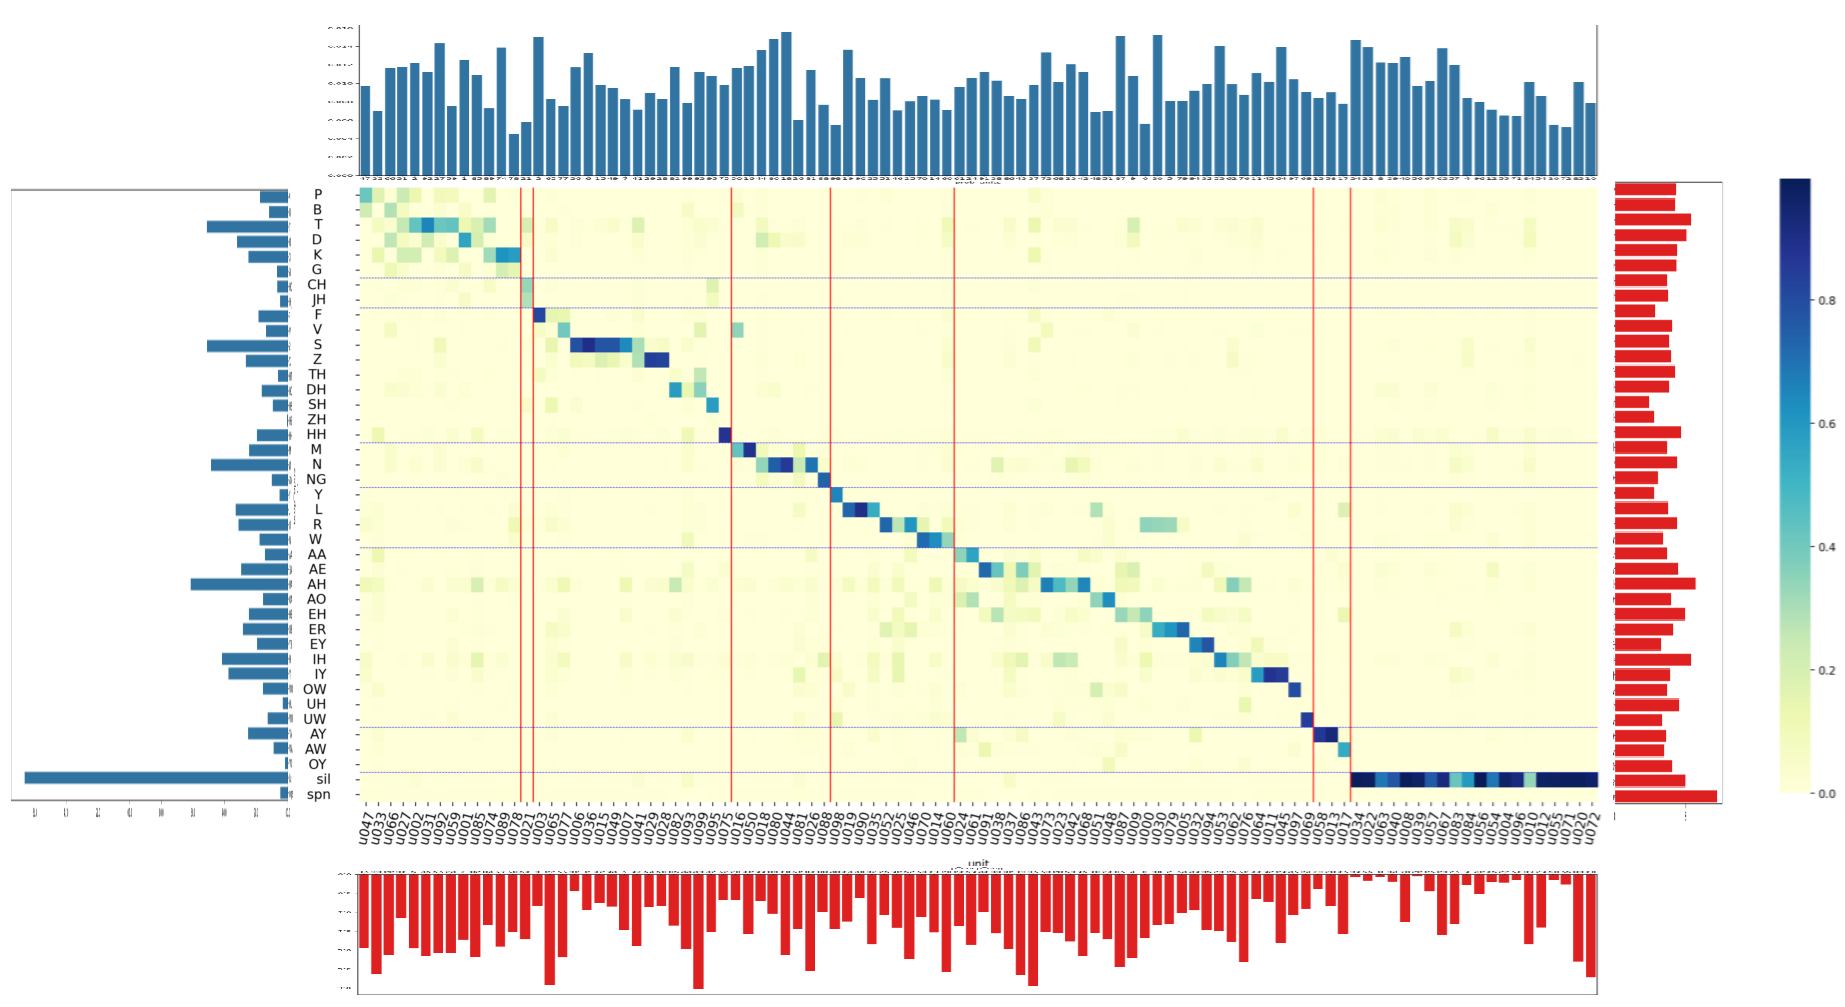
\includegraphics[width=1\linewidth]{figures/better__p_ph_given_un.png}
    \caption{HuBERT 100}
    \label{p_p_given_u-hub-100}
\end{figure}

  為了更直觀的了解模型離散單元與音素之間的對應關係,接下來的分析將把音素與單元的聯合分佈 \(p(p|u)\) 作圖呈現,如 \ref{p_p_given_u-hub-100} 所示。以下說明這張圖表的看法:\par
       橫軸是各單元,而縱軸是各音素,按照發音分組方式,輔音遵循國際音標的圖表排列,元音則按照 ARPABET (cite CMU Dict) 字母順序排列。由於離散單元編號本身並無特殊含義,因此當單元數太多時將省略。\par
       為了更好的看出各組別之間的關係,圖表上先將各組之間以橫線區分。按照語音學分組後,為了考慮單元之間的代表性,將每個單元都找出相對應最高機率的音素,接著將每個單元亦依照對應音素在縱軸的排列順序一一排列,若是遇到對應同一音素的兩種離散單元,則以 \(p(u|p) \) 由高至低排列。最後再橫軸上也以語音學分組區分。\par
       如此一來,便能夠呈現出一張由左上至右下的對應圖。這張圖在 (cite DinoSR) 等 paper 也有呈現。從圖中可以看出,用來編碼 sil 的 unit 其實佔據了不小的部分。